% TRACE-Eval: the paper draft. Build with: latexmk -pdf main   (MiKTeX or TeX Live; pdflatex + bibtex)
% The numbers are those of docs/results/gemma5/report.md; the figure of section 6 is that report's.
\documentclass[11pt,a4paper]{article}
\usepackage[utf8]{inputenc}
\usepackage[T1]{fontenc}
\usepackage{lmodern}
\usepackage[margin=25mm]{geometry}
\usepackage{amsmath,amssymb}
\usepackage{booktabs}
\usepackage{graphicx}
\usepackage{algorithm}
\usepackage{algpseudocode}
\usepackage{tikz}
\usetikzlibrary{positioning,arrows.meta}
\usepackage{microtype}
\usepackage[numbers,sort&compress]{natbib}
\usepackage[hidelinks]{hyperref}
\usepackage{caption}
\captionsetup{font=small}

\newcommand{\strat}[1]{\texttt{#1}}
\newcommand{\Rev}{\mathcal{R}}
\newcommand{\clean}{\textsc{clean}}
\newcommand{\regression}{\textsc{regression}}
\newcommand{\budget}{\textsc{budget}}
\algrenewcommand\algorithmicrequire{\textbf{Input:}}

\title{TRACE-Eval: change-aware, cost-bounded regression test selection\\for LLM agent systems}
\author{Ciprian Păduraru\\University of Bucharest\\\texttt{ciprian.paduraru@unibuc.ro}}
\date{Draft of 10 November 2026}

\begin{document}
\maketitle

\begin{abstract}
An LLM agent system is assembled from skills, prompts, tools, harness code and configuration, and verified by a
suite $T$ of tests whose cost $c(t)$ is dominated by tokens. After a change $\Delta$, a team either reruns all of
$T$ or guesses. We formulate selection, prioritization and stopping as one problem: choose tests from $T$, one at a
time, under a budget $B$, so that the regressions $\Delta$ introduces are found with high probability at low cost.
The change becomes a set of components $C(\Delta)$ (code lines and functions, skill procedures and prose, agent
fields, configuration keys), each broken with a prior probability $\pi_c$. A test's sensitivity
$s_{tc} = P(t\ \text{fails} \mid c\ \text{broken})$ is calibrated from the dependencies observed in execution traces
and from the record of earlier changes, and a test that already fails on the unchanged system, with rate $f_t$, is
discounted. The posterior over the $2^{|C(\Delta)|}$ subsets of broken components is kept exactly; the next test
maximises the expected information gain per token; the run stops with \regression{} at the first failure of a test
that used to pass, with \clean{} when $P(\text{some component broken} \mid \text{outcomes}) < \varepsilon$, and not
before every mandatory property $\Delta$ may affect has been tested. We evaluate on a testbed: a multi-agent
content-operations application whose agents are played by an open model (Gemma~4 E4B), 176 tests, 43 controlled
changes applied as file edits, and a ground truth measured per model by majority over three runs. Declared
dependencies miss 39\% of the regressions; trace-informed selection finds 86\% within 20\% of the full-suite tokens;
two published methods reproduced on the testbed, CASPER's slices and a risk-aware bandit, find 50\% and 59\%
because neither reads the change; the proposed method finds 79\% for 3\% of the tokens, 86\% of the changes that
break a safety property, and gives no false verdict on the 14 changes no test reveals.
\end{abstract}

\section{Introduction}

A platform such as Adobe Experience Manager's agent layer ships dozens of agents. Each is a bundle of a system
prompt, a list of tools, a list of skills (prompt files with a procedure the model follows), and settings, running
on a shared harness that dispatches tool calls, retries, enforces approvals and delegates between agents. The
platform is verified by scenario tests, which run a request end to end and check the final state and the trace,
and by datasets of prompts with expected routings or tool calls. Every test is a run of a model. It costs tokens
and seconds, and the cost varies by a factor of ten to a hundred between a one-shot routing item and a workflow
across five agents.

After a change, the question is the one regression testing has always asked \cite{yoo2012regression}: which tests
to run (selection), in what order (prioritization), and when to stop. Three things make the classic answers
\cite{rothermel1997safe,rothermel2001prioritizing} hard to transfer. Much of the ``code'' is natural language, so
coverage of a skill or a prompt is not a line of a control-flow graph. The outcome of a test is the behaviour of a
model, so it is not a function of the code alone and can vary from run to run. And the cost of a test is not one
unit, so an order that finds a fault after three tests can still have spent a third of the budget.

The literature on efficient evaluation of language models \cite{polo2024tinybenchmarks,li2025atlas,ndzomga2026efficient}
answers a different question: which subset of a benchmark reproduces a score. It selects once, for all models,
and not after a change. The closest work, CASPER \cite{muse2026casper}, is a regression method for LLM-based
systems, but it is change-aware only through drift: it runs representatives of behavioural slices on the new
version and ranks the slices by how much their outcomes moved. Risk-aware adaptive evaluation \cite{maji2026risk}
allocates a budget of runs with a bandit, by impact and by the outcomes seen so far. Neither reads the diff. This
paper's claim is that the diff, mapped to the tests through execution traces, is worth a lot, and that a
sequential Bayesian treatment of the outcomes turns selection, prioritization and stopping into one decision.

The contributions are:
\begin{enumerate}
  \item a formulation of change-aware, cost-bounded testing of agent systems, with the metrics of regression
        testing adapted to token costs (Section~\ref{sec:problem});
  \item a method that extracts a change set at the granularity of code lines, skill procedures, agent fields and
        configuration keys, maps it to tests through dependencies observed in traces, ranks tests by expected
        information per token in a Bayesian model whose sensitivities are calibrated from history, and stops with
        a verdict (Section~\ref{sec:method});
  \item a testbed with a multi-agent application, 176 tests, 43 controlled changes and a mutation-based ground
        truth derived per model, on which strategies are compared by offline replay (Section~\ref{sec:testbed});
  \item an evaluation against six baselines and two published methods reproduced on the testbed
        (Section~\ref{sec:results}).
\end{enumerate}

\section{The problem}
\label{sec:problem}

\paragraph{Objects.}
A system has a current version $V_0$ and a changed version $V_1 = V_0 + \Delta$. The suite $T$ holds tests and
eval items, each with a cost $c(t) > 0$ measured in tokens (prompt and completion tokens over every model call the
test makes). A budget $B$ is a number of tokens, given as a fraction of the cost of the whole suite,
$\sum_{t \in T} c(t)$. Running $t$ on a version $V$ gives an outcome $X_t(V) \in \{\text{pass}, \text{fail}\}$,
which is random because a model produces it. $K$ repetitions on $V_0$ give the baseline fail rate
$f_t = \hat P(X_t(V_0) = \text{fail})$; a test with $f_t \ge \tfrac12$ is one the model already fails, a mistake
of the model rather than a fault of the system.

\paragraph{Ground truth.}
A test $t$ \emph{reveals} $\Delta$ when its majority outcome flips: the pass rate on $V_0$ is at least $\tfrac12$
and the pass rate on $V_1$ is below $\tfrac12$, both over $K$ repetitions. $\Rev(\Delta)$ is the set of revealing
tests; $\Delta$ is a regression when $\Rev(\Delta) \neq \emptyset$. A test the model already fails cannot reveal
anything. The ground truth therefore belongs to the model: a change the model cannot see, because it ignores the
rule with and without the change, is revealed by no test under that model, and a different model may give a
different $\Rev(\Delta)$.

\paragraph{Policies.}
A policy sees the change set $C(\Delta)$, the baseline facts about every test (its traced dependencies, cost and
fail rate), and the outcomes of earlier changes on which it may calibrate, but never $\Rev(\Delta)$. It chooses a
test, observes its outcome and cost on $V_1$, and either chooses again or stops, within $B$. A non-adaptive
policy is an order of $T$ run greedily within the budget. An adaptive one may also return a verdict, \clean{} or
\regression{}, and a probability.

\paragraph{Metrics.}
For a regression, \emph{detection} is whether a revealing test was run and failed, and the \emph{cost to first
detection} is the tokens spent up to that failure. \emph{Tokens spent} is the cost of every test run, on
regressions and on changes that break nothing. A \emph{false alarm} is a failure of a test outside $\Rev(\Delta)$,
which on a change that breaks nothing is a failure the change did not cause. A verdict is \emph{correct} when it
agrees with $\Rev(\Delta) \neq \emptyset$. Prioritization alone, with every test run and no stopping, is scored
by the average percentage of faults detected \cite{rothermel2001prioritizing}. With $n = |T|$, $m = |\Rev(\Delta)|$
and $TF_i$ the position in the order of the test that reveals fault $i$,
\begin{equation}
  \mathrm{APFD} = 1 - \frac{\sum_{i=1}^{m} TF_i}{n\,m} + \frac{1}{2n},
\end{equation}
which is near 1 when the first tests find every fault and near 0 when the last ones do; a random order scores
about $\tfrac12$. Because costs differ by an order of magnitude, we read its cost-cognizant form
\cite{elbaum2001incorporating,malishevsky2006cost}. With $c_j$ the cost of the $j$-th test in the order,
$C = \sum_j c_j$, and $\sigma_i$ the severity of fault $i$ (the risk weight of its revealing test, 1 to 4),
\begin{equation}
  \mathrm{APFD}_c = \frac{\sum_{i=1}^{m} \sigma_i \big( C - \sum_{j < TF_i} c_j - \tfrac12 c_{TF_i} \big)}
                         {C \sum_{i=1}^{m} \sigma_i}.
\end{equation}
Finding a fault after a few cheap tests costs little and scores high; finding it after the long workflows scores
low, however few tests came before. An order can score well on APFD and poorly on $\mathrm{APFD}_c$ by putting
the expensive tests first.

\section{Overview}
\label{sec:overview}

Figure~\ref{fig:overview} follows one change from the diff to a verdict. Three inputs exist before the change is
tested: the diff, which becomes a change set; a traced full run of the current version, which gives every test
its observed dependencies, its cost and its pass rate; and the earlier changes whose full-suite outcomes are
known, which calibrate how often a test that touches a changed component of a given kind actually reveals the
change. From these the model assigns a prior to every changed component and a sensitivity to every (test,
component) pair. The loop then picks the test with the most expected information per token, runs it on the
changed version, updates the posterior over the subsets of broken components, and repeats until a stopping rule
fires: a failure of a test that used to pass, a posterior probability of any breakage below $\varepsilon$, or an
exhausted budget. A run that found nothing does not end before every mandatory property the change may affect has
a test. In a team's pipeline the nightly full-suite runs supply the traced baseline and the record of earlier
changes; a pull request supplies the diff.

\begin{figure}[t]
  \centering
  \resizebox{\textwidth}{!}{% The end-to-end overview (Figure 1 of main.tex). No numbers on the figure: it shows the mechanism, not a result.
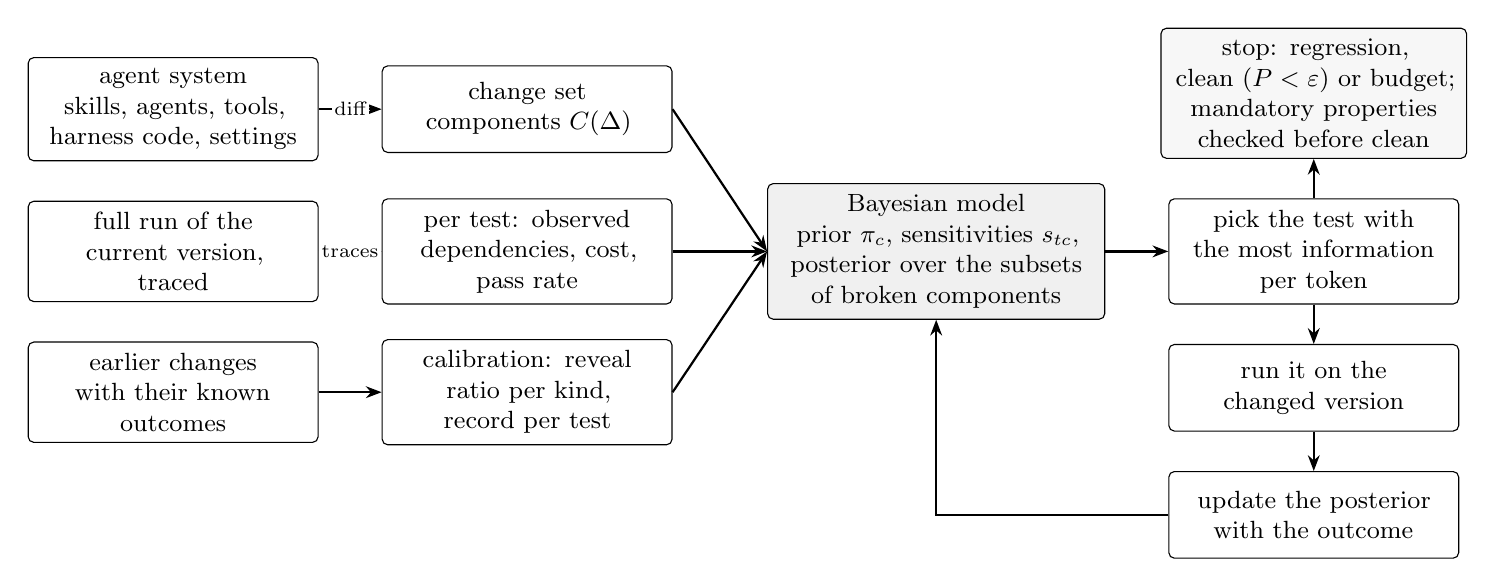
\begin{tikzpicture}[
  node distance=5mm and 8mm,
  box/.style={draw, rounded corners=2pt, align=center, font=\small, inner sep=4pt, minimum height=11mm, text width=34mm},
  model/.style={box, fill=black!6, text width=40mm, minimum height=16mm},
  stop/.style={box, text width=36mm, fill=black!3},
  arr/.style={-{Stealth[length=2mm]}, thick},
  lbl/.style={font=\scriptsize, fill=white, inner sep=1pt}
]
% inputs, left column
\node[box] (sys) {agent system\\skills, agents, tools,\\harness code, settings};
\node[box, below=of sys] (run) {full run of the\\current version,\\traced};
\node[box, below=of run] (hist) {earlier changes\\with their known\\outcomes};
% what the inputs become, middle-left column
\node[box, right=of sys] (cs) {change set\\components $C(\Delta)$};
\node[box, right=of run] (deps) {per test: observed\\dependencies, cost,\\pass rate};
\node[box, right=of hist] (cal) {calibration: reveal\\ratio per kind,\\record per test};
% the model and the loop
\node[model, right=12mm of deps] (bayes) {Bayesian model\\prior $\pi_c$, sensitivities $s_{tc}$,\\posterior over the subsets\\of broken components};
\node[box, right=of bayes] (pick) {pick the test with\\the most information\\per token};
\node[box, below=of pick] (exec) {run it on the\\changed version};
\node[box, below=of exec] (upd) {update the posterior\\with the outcome};
\node[stop, above=of pick] (stop) {stop: regression,\\clean ($P<\varepsilon$) or budget;\\mandatory properties\\checked before clean};
% edges
\draw[arr] (sys) -- node[lbl] {diff} (cs);
\draw[arr] (run) -- node[lbl] {traces} (deps);
\draw[arr] (hist) -- (cal);
\draw[arr] (cs.east) -- (bayes.west);
\draw[arr] (deps.east) -- (bayes.west);
\draw[arr] (cal.east) -- (bayes.west);
\draw[arr] (bayes) -- (pick);
\draw[arr] (pick) -- (exec);
\draw[arr] (exec) -- (upd);
\draw[arr] (upd.west) -| (bayes.south);
\draw[arr] (pick) -- (stop);
\end{tikzpicture}
}
  \caption{From a diff to a verdict. The three inputs on the left exist before the change is tested: the diff,
  a traced run of the current version, and earlier changes with their known outcomes. The loop on the right
  runs one test at a time on the changed version.}
  \label{fig:overview}
\end{figure}

\section{Methods}
\label{sec:method}

\subsection{What a diff becomes}

The change-set extractor compares the current and the changed trees and emits \emph{components} with the
identifiers the dependency model uses: \texttt{code:<file>::<function>} for a function whose normalised syntax
tree changed, \texttt{line:<file>:<n>} for each changed line of code, \texttt{tool:<name>} when the function is a
registered tool adapter, \texttt{skill:<name>\#procedure}, \texttt{\#prose} or \texttt{\#meta} for the three
parts of a skill file, \texttt{agent:<name>.<field>} for a changed field of an agent definition (an agent's tool
or skill list that only lost items names them), \texttt{config:<key>} for a changed effective setting, and
\texttt{fixture:<name>}. Comments, docstrings, blank lines, formatting and the order of configuration mappings add
nothing: no component, no file and no diff line, so no policy and no probability can depend on them. Skill files
are prompts the model reads word for word, so all of their text counts.

\subsection{Dependencies}

\emph{Declared} dependencies are the metadata a test's author wrote. They are incomplete on purpose, as in
practice: shared skills reached through an include, harness code and most configuration keys are not declared.
\emph{Observed} dependencies come from the traced baseline runs: the agents started, the agent fields the
orchestrator consulted, the skills loaded, the tools called, the configuration keys read, and the code functions
and lines executed, with a dynamic coverage context per test and repetition. For a test $t$ and a dependency $d$,
$\phi_t(d) \in [0, 1]$ is the share of $t$'s baseline runs that exercised $d$. A component matches a dependency
set when the set holds the component, its base (\texttt{skill:x} for \texttt{skill:x\#procedure}), or a function of
a module changed at module level.

\subsection{Baselines}

Six strategies span the design space of the literature. All see the same inputs as the method.
\begin{itemize}
  \item \strat{full}: the suite in catalog order (the reference). \strat{random}: a random permutation.
  \item \strat{declared}: the tests whose declared dependencies match a changed component, by risk then
        affinity then cost; classic selection on metadata \cite{rothermel1997safe}.
  \item \strat{ir\_tfidf}: every test ranked by the TF-IDF cosine between the text of the change (file names,
        component ids, the diff of the code) and the text of the test (name, request, expectations), as in REPiR
        \cite{saha2015ir}. It uses no traces.
  \item \strat{observed}: the tests whose observed dependencies match a changed component, scored by
        $a_t \cdot \rho_t / c(t)$, where $a_t$ is the affinity (the matching components weighted by
        $\phi_t$; line hits count once per file) and $\rho_t$ the risk weight. Trace-informed selection.
  \item \strat{cost\_aware}: the whole suite ranked by $\rho_t\,(0.05 + a_t + [\text{line hit}])\,(2 - p_t) / c(t)$,
        with $p_t$ the baseline pass rate: affected tests first, cheap ones before expensive ones, and the
        unaffected tests after them so that the budget is used \cite{elbaum2001incorporating,memon2017taming}.
\end{itemize}
Two optional baselines, predictive selection with a logistic model over the same features
\cite{machalica2019predictive} and a diversity-based order \cite{pan2024ltm}, are in the code and not in the
tables.

\subsection{The proposed method}

\paragraph{Hypotheses.}
Each changed component $c \in C(\Delta)$ is broken with a prior $\pi_c$ that depends on its kind: about $0.45$ to
$0.5$ for code, skill procedures, configuration and agent fields, $0.12$ to $0.15$ for prompt wording and skill
prose. Tool and line components are views of a code change, not separate causes, and are folded into it. The
posterior is kept exactly over all $2^k$ subsets $h \in \{0,1\}^{C(\Delta)}$, with $k \le 8$ (the likeliest
components are kept when there are more).

\paragraph{Likelihood.}
A test passes only if it would pass on the current version and none of the broken components makes it fail:
\begin{equation}
  q_t(h) = P(t\ \text{fails} \mid h) = 1 - (1 - f_t) \prod_{c:\, h_c = 1} (1 - s_{tc}).
  \label{eq:likelihood}
\end{equation}
A test the model already fails ($f_t$ near 1) fails under every hypothesis, so its outcome carries no
information, which is what keeps the method from mistaking the model's mistakes for regressions.

\paragraph{Sensitivity.}
Covering a component is weak evidence by itself: most tests that execute a changed function do not fail when it
breaks. The sensitivity is therefore calibrated (Algorithm~\ref{alg:sens}) from the earlier changes whose outcomes
are known, never from the change under test:
\begin{equation}
  s_{tc} = \mathrm{clip}\big(r_{k(c)} \cdot \ell_{t,k(c)} \cdot \phi_t(c) \cdot \tau_t,\ 0.02,\ 0.9\big),
  \label{eq:sens}
\end{equation}
where $r_k$ is the reveal ratio of the component's kind $k$ (among the tests that statically looked impacted by
earlier changes of that kind, the share that revealed them, with the kinds separating a test that executed a
changed line from one that only called the changed function, and agent fields calibrated per field);
$\ell_{tk} = (O_{tk} + m) / (E_{tk} + m)$ is the test's own lift on that kind, with $O_{tk}$ the earlier changes
of kind $k$ it revealed, $E_{tk}$ the number an average impacted test would have revealed (the sum of those
changes' reveal rates), and $m = 2$ a padding that keeps a short record from moving the lift far; $\phi_t(c)$ is
how often the baseline runs exercised the component, or, for an agent that lost tools or skills, how often $t$
used one of the lost items; and $\tau_t \in [0.5, 2]$ tilts the sensitivity up for a test whose text shares
vocabulary with the diff and for one whose author declared the dependency. The lift matters because a change
that breaks most of the suite says little about each test it breaks, while a change that one test alone caught
says a lot about that test. A test with no link to the component gets a small constant $s_{\mathrm{ind}} = 0.02$;
one declared but never observed gets half the kind's ratio.

\paragraph{Policy, stopping and the mandatory rule.}
Algorithm~\ref{alg:adaptive} runs the loop. The next test maximises the expected reduction of the posterior's
entropy \cite{lindley1956measure}, tilted by risk, per token. After a pass, tests that behave exactly like the
one that passed (same agents, tools, fault profile and dataset in the baseline) have their sensitivities
discounted by $\delta = 0.35$, because near-duplicates give correlated evidence rather than independent draws.
Each test runs at most once: the models decode greedily, so a rerun would almost always repeat the answer. The
run stops with \regression{} at the first failure of a test that passed on the current version, because under
greedy decoding that failure is a changed behaviour, which is what the ground truth calls revealing. It stops
with \clean{} when $1 - P(h = \mathbf{0}) < \varepsilon$, with $\varepsilon = 0.05$, and otherwise when the budget
is spent or no test can still move the posterior. Before a run ends without a regression, every mandatory
property the change may affect (the properties whose sources the change touches, and those of the tests that ran
a changed component on the current version) gets a test if it has none yet: the cheapest test of that property
that passes on the current version, while the budget allows. A failure there is a regression like any other.

\begin{algorithm}[H]
\caption{Adaptive Bayesian selection with stopping}
\label{alg:adaptive}
\begin{algorithmic}[1]
\Require components $C(\Delta)$ with priors $\pi_c$; tests $T$ with costs $c(t)$, fail rates $f_t$, risk tilts
  $\rho_t$ and sensitivities $s_{tc}$ (Algorithm~\ref{alg:sens}); near-duplicate groups; budget $B$; $\varepsilon$, $\delta$
\State $P(h) \propto \prod_{c} \pi_c^{h_c} (1 - \pi_c)^{1 - h_c}$ for $h \in \{0,1\}^{C(\Delta)}$
  \Comment{$h = \mathbf{0}$: nothing is broken}
\State $q_t(h) \gets 1 - (1 - f_t) \prod_{c:\, h_c = 1} (1 - s_{tc})$ for every $t$ and $h$
  \Comment{Equation~\ref{eq:likelihood}}
\State $R \gets \emptyset$;\ $b \gets B$
\Loop
  \If{$1 - P(\mathbf{0}) < \varepsilon$} \State \Return \textsc{Finish}(\clean) \EndIf
  \State $p_t \gets \sum_h P(h)\, q_t(h)$ \Comment{$P(t$ fails$)$ under the posterior}
  \State $g_t \gets H(P) - p_t\, H(P \mid t\ \text{fails}) - (1 - p_t)\, H(P \mid t\ \text{passes})$
    \Comment{expected information gain}
  \State $t^\star \gets \arg\max\{\, g_t\, \rho_t / c(t) : t \notin R,\ c(t) \le b,\ g_t > 0 \,\}$
  \If{there is no such $t^\star$} \State \Return \textsc{Finish}(\budget) \EndIf
  \State run $t^\star$ on $V_1$: outcome $x$, cost $\kappa$;\ $R \gets R \cup \{t^\star\}$;\ $b \gets b - \kappa$
  \State $P(h) \gets P(h)\, q_{t^\star}(h)$ if $x = \text{fail}$, else $P(h)\,(1 - q_{t^\star}(h))$; normalise
  \If{$x = \text{fail}$ and $f_{t^\star} < \tfrac12$} \State \Return \regression{}
    \Comment{a test that used to pass has failed}
  \EndIf
  \If{$x = \text{pass}$}
    \State $s_{uc} \gets \delta\, s_{uc}$ and recompute $q_u$ for every unrun $u$ in the group of $t^\star$
  \EndIf
\EndLoop
\Statex
\Procedure{Finish}{verdict}
  \ForAll{mandatory properties $p$ the change may affect, in id order}
    \If{no test in $R$ checks $p$}
      \State $u \gets$ the cheapest $u \notin R$ with $p \in \mathrm{props}(u)$, $f_u < \tfrac12$, $c(u) \le b$;
        \textbf{continue} if none
      \State run $u$; $R \gets R \cup \{u\}$; $b \gets b - \kappa$; update $P$ as above
      \If{$u$ failed} \State \Return \regression{} \EndIf
    \EndIf
  \EndFor
  \State \Return verdict, with $1 - P(\mathbf{0})$
\EndProcedure
\end{algorithmic}
\end{algorithm}

\begin{algorithm}[H]
\caption{Calibration of the sensitivities from the earlier changes}
\label{alg:sens}
\begin{algorithmic}[1]
\Require earlier changes $\mathcal{D}$ with their revealing sets $\Rev(\Delta')$; defaults $r^0_k$ per kind;
  padding $m$; the change under test $\Delta \notin \mathcal{D}$
\ForAll{$\Delta' \in \mathcal{D}$ and components $c' \in C(\Delta')$ of kind $k$}
  \State $I \gets$ the tests that look impacted by $c'$: executed a changed line, called the changed function,
    or match the component
  \State $\mathrm{rate} \gets |\Rev(\Delta') \cap I| / |I|$;\ append $\mathrm{rate}$ to $A_k$
  \State $O_{tk} \mathrel{+}= [t \in \Rev(\Delta')]$ and $E_{tk} \mathrel{+}= \mathrm{rate}$ for $t \in I$
    \Comment{once per change and kind}
\EndFor
\State $r_k \gets \mathrm{clip}\big((\sum A_k + m\, r^0_k) / (|A_k| + m),\ 0.01,\ 0.9\big)$ for every kind $k$
\ForAll{tests $t$ and components $c \in C(\Delta)$ of kind $k$}
  \State $\ell_{tk} \gets (O_{tk} + m) / (E_{tk} + m)$;\quad
    $\tau_t \gets 0.5 + \mathrm{text}(t, \Delta) + 0.5\,[\text{declared}]$
  \State $s_{tc} \gets \mathrm{clip}(r_k\, \ell_{tk}\, \phi_t(c)\, \tau_t,\ 0.02,\ 0.9)$ if $\phi_t(c) > 0$;\
    $\tfrac12 r_k$ if declared only;\ $s_{\mathrm{ind}}$ otherwise
\EndFor
\end{algorithmic}
\end{algorithm}

\paragraph{Order for the prioritization metrics.}
APFD and $\mathrm{APFD}_c$ score a complete order. The method's order is the greedy sequence it would pick if every
test passed, with no stopping, followed by the untouched tests in cost-aware order.

\subsection{Two published methods, reproduced}

CASPER \cite{muse2026casper} and risk-aware adaptive evaluation \cite{maji2026risk} are the closest published
methods. Both are reproduced on the testbed (Algorithms~\ref{alg:casper} and \ref{alg:bandit}) with the
adaptations the setting forces, which the code documents. Neither reads the diff, so comparing with them isolates
what change-awareness adds.

CASPER mines ten behavioural signals from the logs of the current version, cuts the suite into slices that are
coherent in signal space and consistent in outcome, runs a few representatives of every slice on the new version,
and ranks the slices by how much a model of the signals changed its prediction. Here the signals are the
counterparts for an agent that calls tools and hands off to other agents (turns, tool calls, distinct tools, the
share of the most-called tool, the entropy of the calls, hand-offs, skills loaded, settings read, the size of the
run and the share the model wrote); the slices come from k-means \cite{lloyd1982least} on the standardised signals
with the baseline outcome as a heavier column, in place of the paper's evolutionary search; two representatives
per slice run first, cheapest slices first; and, because the replay oracle returns an outcome and a cost rather
than a trace, a slice is scored by the shift of its representatives' failure rate.

Risk-aware adaptive evaluation is a contextual Thompson-sampling bandit \cite{thompson1933likelihood,chapelle2011empirical}:
a scenario's context is a vector of features of its definition, its impact a fixed score, the reward of a trial
impact times failure. Each round, a logistic regression on every outcome so far gives every scenario a failure
probability; a Beta posterior per scenario mixes it, with weight $\lambda$, with the scenario's own outcomes;
one draw per scenario, times the impact, picks the next. Here the scenarios are the tests, the context is the
case's definition and the shape of its baseline runs, the impact is the risk weight, the budget is in tokens and
each test runs once. As in the paper, any failure is a reward, so a test the model already fails counts as a
find, and there is no stopping rule and no verdict.

\begin{algorithm}[H]
\caption{CASPER's slices, reproduced}
\label{alg:casper}
\begin{algorithmic}[1]
\Require baseline runs of every test; slice size $n_s$, minimum size $n_{\min}$, outcome weight $w$,
  representatives $K$; budget $B$
\State $Z \gets$ the standardised behavioural signals of every test, with $w \cdot$ (standardised pass rate) as an
  extra column
\State slices $\gets$ k-means$(Z, \lceil |T| / n_s \rceil)$; merge every slice smaller than $n_{\min}$ into the
  slice whose centre is nearest
\ForAll{slices $j$} \State $\mathrm{reps}_j \gets$ the member nearest the centre, then farthest-point sampling,
  $K$ in all \EndFor
\State run the representatives of every slice on $V_1$, cheapest slices first, while the budget allows
\State $\mathrm{shift}_j \gets$ failure rate of $\mathrm{reps}_j$ on $V_1$ minus their baseline failure rate
\State order the slices: $\mathrm{shift} > 0$ by size, then $\mathrm{shift} < 0$, then unchanged
\State run the members of each slice in that order, nearest the centre first, until the budget is spent
\end{algorithmic}
\end{algorithm}

\begin{algorithm}[H]
\caption{Risk-aware adaptive evaluation, reproduced}
\label{alg:bandit}
\begin{algorithmic}[1]
\Require context $x_t$ of every test (standardised, with an intercept), impact $\iota_t$, costs $c(t)$;
  mixing weight $\lambda$, ridge penalty $\lambda_2$; budget $B$
\State $n_t \gets 0$, $k_t \gets 0$ for every $t$;\ $b \gets B$
\State run a test chosen uniformly at random among those with $c(t) \le b$
\While{some unrun $t$ has $c(t) \le b$}
  \State $w \gets \arg\min_w \sum_{t:\, n_t > 0} \mathrm{logloss}(\sigma(w^\top x_t), k_t) + \tfrac{\lambda_2}{2}\|w\|^2$
    \Comment{Newton's method, warm start}
  \State $p_t \gets \sigma(w^\top x_t)$;\quad
    $\theta_t \sim \mathrm{Beta}\big(1 + \lambda p_t + k_t,\ 1 + \lambda (1 - p_t) + n_t - k_t\big)$ for every
    unrun $t$ that fits
  \State run $t^\star \gets \arg\max_t \iota_t\, \theta_t$ on $V_1$; $n_{t^\star} \gets 1$; $k_{t^\star} \gets
    [\text{failed}]$; $b \gets b - \kappa$
\EndWhile
\end{algorithmic}
\end{algorithm}

\section{The testbed}
\label{sec:testbed}

\paragraph{The application.}
ContentOps is a content-operations platform in the style of a web content manager: pages with versions, assets,
publishing with reviews and schedules, link validation, SEO metadata, translation, governance with consent and
approval tokens, rollback, brand rules, analytics and a site audit. Eleven agents (an orchestrator and ten
specialists, three of them modelled on Adobe's) run on a shared harness with thirteen skills and 32 tools over
deterministic services. The orchestrator delegates a request to one specialist or, when it needs several, plans
the steps and asks a person before any step that publishes, schedules or takes pages down. The structure is
deliberate: some components are shared with a wide blast radius (a governance skill included by several skills,
a permission check available to eight specialists, a retry helper around every tool call), others are narrow,
and some policies are enforced only in a skill while others also in a tool. The agents are played by a real
model, Gemma~4 E4B, served with vLLM and decoding greedily.

\paragraph{The suite.}
The recording holds 176 cases: scenario tests, fifteen of which run one of six multi-agent workflows end to end,
and the items of two datasets (prompt to expected delegation, prompt to expected tool call). A case defines its
entry agent, request, fixture and fault profile (healthy, one transient failure of a tool, one lost
acknowledgement, a tool permanently down), a risk level (critical to low, weights 4 to 1), the properties it
checks, declared dependencies, and expectations on the final state, the tools required and forbidden, attempt
and audit counts, the answer, the step limit and the order of agents and tools. The properties come from a
catalog of fifteen (correctness, safety, resilience, orchestration, efficiency, quality), each with how it is
checked, a threshold and a mandatory flag; the six safety properties are mandatory. A model can draft the
catalog from the requirements alone, for a person to edit. A judge model reads the answer only for the two cases
with a rubric, and only after the deterministic checks pass.

\paragraph{The changes.}
Forty-three controlled changes are applied as file edits (Table~\ref{tab:changes}), in the spirit of mutation
analysis \cite{demillo1978hints,jia2011analysis}: ten to tool adapters, services and the harness, three to the
runtime loop, eleven to skills, two to agent definitions, seven to configuration, one combined change whose two
halves are harmless alone, and nine benign changes. A change has to touch an input a model acts on, and a removed
step has to go from both the procedure and the prose of a skill, or the model does the step anyway. Candidates
that told nothing about selection were left out: twins of other changes, crashes, and a change that broke most of
the suite. Ten of the changes aim at the workflows.

\begin{table}[t]
\centering\small
\caption{The 43 controlled changes.}
\label{tab:changes}
\begin{tabular}{lrp{98mm}}
\toprule
category & count & examples \\
\midrule
code & 10 & argument swap in a tool adapter; retries drop idempotency keys; approval gate bypassed; external links treated as reachable; a shared read reports the wrong review flag; ranking sorted the wrong way; case-sensitive search and brand check \\
runtime & 3 & the agent loop stops six steps early; a delegated answer is truncated; a delegation drops the ids of earlier steps \\
skill & 11 & publishing drops link validation or the permission check; authoring drops its metadata step; translation hard-codes a default; rollback restores the wrong version; governance drops the consent check; the routing skill stops asking for approval, or drops the brand gate \\
agent definition & 2 & an agent loses a tool \\
configuration & 7 & link validation disabled; review not required; a step budget of five; no retries; a title limit of twenty; another default agent; no approval needed to take a page down \\
combined & 1 & a keyword rule in code and a very low limit in configuration \\
benign & 9 & prose reflowed or reworded; a comment or docstring edited; local variables renamed; configuration comments reordered; an unused tool added; prompt wording; lists reordered \\
\bottomrule
\end{tabular}
\end{table}

\paragraph{Protocol.}
The full suite runs $K = 3$ times on the current version with coverage contexts, which gives the observed
dependencies, costs and pass rates, and $K = 3$ times on each of the 43 changed copies, which gives the ground
truth. Every strategy is then replayed offline: for every change, budget in $\{2, 5, 10, 20, 30, 50, 100\}\%$ of
the full-suite tokens and five seeds, the strategy sees the baseline facts and the change set, and each test it
runs is answered from a recorded run of that changed copy. The method calibrates on the other 42 changes, never
on the one under test. The environment's failures (a server that did not answer) are marked and left out, as if
the run had not been made.

\section{Results}
\label{sec:results}

\paragraph{Ground truth.}
On the current version 170 of 176 tests pass. The six failures are the model's own mistakes, which clearer
wording did not fix: it schedules a page without an approved review, requests a review nobody asked for, applies
an over-long title, goes on to publishing after a failed link check, and stops a whole plan after a refused step
the other steps do not depend on. Of the 34 regressions, 29 are revealed by at least one test. The model does not
act on the five remaining guards (a review flag, a length limit, a non-blocking asset reference) with or without
the change, so it behaves the same, wrongly, on both versions. No benign change fails a test. Across the 43
changes the three runs disagreed on five (change, test) pairs, which the majority vote absorbs. The 29 revealed
regressions and the 14 changes no test reveals are the population below.

\begin{table}[t]
\centering\small
\caption{Detection of the 29 revealed regressions by nominal budget (share of the full-suite tokens), and the
tokens actually spent: on regressions at a 20\% and a 100\% budget, and on the benign changes at 100\%.
Five seeds; the last three columns are shares of the full-suite tokens.}
\label{tab:detection}
\begin{tabular}{lcccccc ccc}
\toprule
strategy & 2\% & 5\% & 10\% & 20\% & 50\% & 100\% & spent@20 & spent@100 & benign@100 \\
\midrule
\strat{full}            & 0.00 & 0.14 & 0.21 & 0.34 & 0.90 & 0.99 & 0.20 & 0.98 & 1.00 \\
\strat{random}          & 0.17 & 0.21 & 0.33 & 0.52 & 0.84 & 0.99 & 0.20 & 0.98 & 1.00 \\
\strat{declared}        & 0.45 & 0.55 & 0.55 & 0.61 & 0.61 & 0.61 & 0.07 & 0.10 & 0.13 \\
\strat{ir\_tfidf}       & 0.59 & 0.70 & 0.71 & 0.92 & 0.99 & 0.99 & 0.20 & 0.98 & 0.99 \\
\strat{observed}        & 0.48 & 0.62 & 0.69 & 0.86 & 0.86 & 0.99 & 0.15 & 0.49 & 0.32 \\
\strat{cost\_aware}     & 0.38 & 0.59 & 0.62 & 0.83 & 0.86 & 0.99 & 0.20 & 0.98 & 0.99 \\
\strat{casper\_slices}  & 0.17 & 0.28 & 0.43 & 0.50 & 0.88 & 0.99 & 0.20 & 0.98 & 1.00 \\
\strat{risk\_aware\_ts} & 0.12 & 0.27 & 0.43 & 0.59 & 0.81 & 0.99 & 0.20 & 0.98 & 1.00 \\
\strat{adaptive\_bayes} & 0.59 & 0.76 & 0.79 & 0.79 & 0.83 & 0.83 & 0.03 & 0.03 & 0.20 \\
\bottomrule
\end{tabular}
\end{table}

\begin{table}[t]
\centering\small
\caption{Order quality and verdicts. APFD and $\mathrm{APFD}_c$ of the complete order; cost to the first true
detection as a share of the full suite (detected cases); detection of the 21 regressions that break a safety
property at a 10\% and a 20\% budget; share of replays, over all budgets, in which the strategy saw a failure on
one of the 14 changes no test reveals.}
\label{tab:order}
\begin{tabular}{lccc cc c}
\toprule
strategy & APFD & $\mathrm{APFD}_c$ & first detection & safety@10 & safety@20 & false alarm \\
\midrule
\strat{full}            & 0.63 & 0.57 & 0.19 & 0.10 & 0.24 & 0.71 \\
\strat{random}          & 0.56 & 0.53 & 0.14 & 0.36 & 0.57 & 0.63 \\
\strat{declared}        & 0.81 & 0.76 & 0.025 & 0.52 & 0.55 & 0.51 \\
\strat{ir\_tfidf}       & 0.78 & 0.77 & 0.040 & 0.79 & 0.98 & 0.70 \\
\strat{observed}        & 0.75 & 0.79 & 0.048 & 0.57 & 0.81 & 0.57 \\
\strat{cost\_aware}     & 0.75 & 0.78 & 0.056 & 0.57 & 0.76 & 0.91 \\
\strat{casper\_slices}  & 0.59 & 0.54 & 0.12 & 0.50 & 0.60 & 0.57 \\
\strat{risk\_aware\_ts} & 0.60 & 0.61 & 0.13 & 0.55 & 0.73 & 0.71 \\
\strat{adaptive\_bayes} & 0.83 & 0.81 & 0.017 & 0.86 & 0.86 & 0.00 \\
\bottomrule
\end{tabular}
\end{table}

\begin{figure}[t]
  \centering
  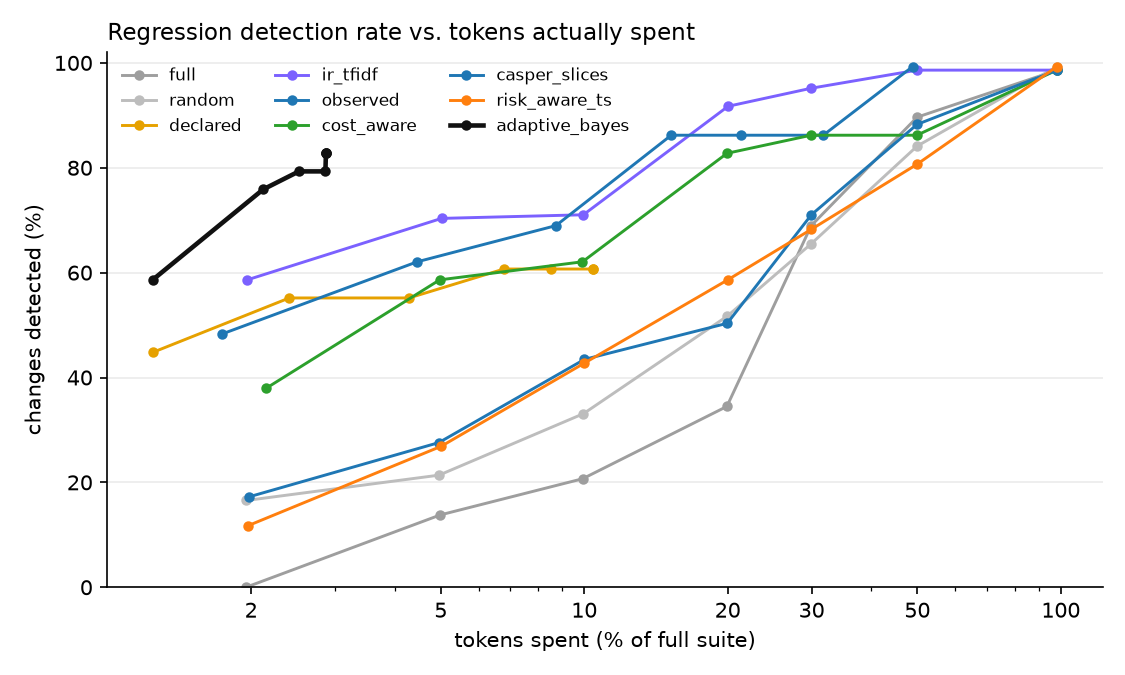
\includegraphics[width=0.85\textwidth]{../results/gemma5/figures/detection_vs_cost.png}
  \caption{Detection of the 29 revealed regressions against the tokens actually spent, every strategy and
  budget. The adaptive method sits at the left: it stops.}
  \label{fig:detection}
\end{figure}

\paragraph{Selection (RQ1, RQ2).}
Declared metadata caps detection at 61\% however large the budget (Table~\ref{tab:detection}), because shared
skills reached through an include, harness code and most configuration keys are not declared. The observed
dependencies recover full selection recall at half the suite's cost and reach 86\% within a 20\% budget. The
argument for trace-informed selection holds.

\paragraph{Prioritization (RQ3).}
The informed strategies raise $\mathrm{APFD}_c$ from 0.53 (random) to 0.76--0.81 (Table~\ref{tab:order}). The
adaptive method's order is the best and finds the first regression soonest, after 1.7\% of the suite's tokens.
The two reproduced methods order no better than random (0.54 and 0.61) and find their first regression after
12--13\% of the suite, where the change-aware strategies need 2--6\%.

\paragraph{Budget (RQ4).}
The adaptive method is the only strategy that returns budget. It finds 76\% of the regressions at a 5\% budget
and 79\% at 20\%, for under 3\% of the tokens, and spends a tenth of the suite on a benign change at a 20\%
budget (Figure~\ref{fig:detection}). TF-IDF over the diff is the strongest selector at 20\% (92\%) and the
strongest on the safety-breaking changes (98\%), and it spends the whole budget every time, on benign changes
too. The adaptive method's ceiling is 83\%: on a regression that only one to five tests reveal it can become
confident that nothing broke before reaching them (145 of 1,015 replays of regressions ended \clean). The changes
it misses at 20\% are the delegation that drops the ids of earlier steps, the loop that stops six steps early,
retries without idempotency keys, the routing skill without its brand gate, the authoring skill without its
metadata step, and the combined change, which runs out of budget.

\paragraph{Verdicts and the model's own mistakes.}
The six tests that fail on the current version fail on every changed copy too. A strategy that runs one sees a
failure the change did not cause: on the 14 changes no test reveals, this happens to \strat{full} in 71\% of its
replays, to \strat{cost\_aware} in 91\%, to the bandit in 71\% and to CASPER's slices in 57\%
(Table~\ref{tab:order}). The adaptive method discounts a test by its failures on the current version
(Equation~\ref{eq:likelihood}) and stops only on a test that used to pass, so it gave no \regression{} verdict on
any of these changes in 490 replays.

\paragraph{The text factor.}
The tilt $\tau_t$ can use word overlap (the default), the TF-IDF similarity of \strat{ir\_tfidf}, or no text at
all (Table~\ref{tab:text}). TF-IDF brings forward the one test that reveals a narrow change and gains up to four
points while spending less; without any text the method loses ten points. Text matters, and coverage and history
carry most of the result. The testbed is textual, since tests, skills and configuration keys share vocabulary,
which favours any text measure.

\begin{table}[t]
\centering\small
\caption{Detection by the method with three text measures, with the tokens spent in parentheses, against
\strat{ir\_tfidf} alone.}
\label{tab:text}
\begin{tabular}{lcccc}
\toprule
budget & word overlap & TF-IDF & no text & \strat{ir\_tfidf} alone \\
\midrule
5\%  & 0.76 (2.1\%) & 0.79 (2.0\%) & 0.62 (2.4\%) & 0.70 (5\%) \\
20\% & 0.79 (2.9\%) & 0.83 (2.4\%) & 0.69 (3.5\%) & 0.92 (20\%) \\
50\% & 0.83 (2.9\%) & 0.83 (2.4\%) & 0.69 (4.5\%) & 0.99 (50\%) \\
\bottomrule
\end{tabular}
\end{table}

\paragraph{The mandatory rule.}
Without the rule, a run that found no regression had tested every mandatory property the change may affect in
33\% of the replays at a 20\% budget; with it, in 90\%, for 0.8 extra tests per change on average, and detection
rose from 76\% to 79\%. The rule is also a detector: it catches the publishing skill without its link validation,
which the model alone calls clean, because the method must test the mandatory property ``no broken publish''
before ending, and that test fails. The rule never caused a false verdict. Below a 10\% budget it often cannot
afford the extra test.

\paragraph{The reproduced methods, and where CASPER fits.}
CASPER's slices and the risk-aware bandit find 50\% and 59\% of the regressions at a 20\% budget, between random
(52\%) and the change-aware strategies (83--92\%). The bandit's impact is the test's risk, so it does better on
the changes that break a safety property (73\% at 20\%, 94\% at 50\%), and it rewards any failure, so it runs the
model's red tests early. Neither stops. These numbers measure what the diff is worth, not CASPER in its own
setting. CASPER was built for changes that have no diff a test can be mapped to: a model upgrade, a provider's
silent update, a prompt-level change whose effect spreads through the model's behaviour. It needs only the logs
of the last full run, so it applies to a system whose code the testing team does not own, and its cost does not
grow with the suite, since a fixed number of representatives per slice samples a large suite as cheaply as a
small one. A platform sees both kinds of change. The change-aware strategies cover the edits to skills, code and
settings; CASPER's representatives are the natural first pass after a model update, when every test is affected
and the question is which behaviours drifted. The two could be combined: the slices can serve as the
near-duplicate groups of the adaptive method, and a slice whose representatives drifted can enter the model as a
changed component. On this testbed every change is an edit with a diff and the suite is small (176 tests, twelve
slices), which is the case slicing has least to offer.

\paragraph{Other models.}
The same application was recorded with Qwen3.8-27B and with gpt-oss-120b, served as they are, with greedy
decoding. Neither recording is a clean ground truth. Qwen passes 171 of the 176 tests on the current version
and reveals every regression, but it also ``reveals'' every benign change, by two to five tests, including a
change whose change set is empty: six tests answer differently when they run 64 at a time, as the changed copies
do, than one at a time, as the baseline does, and its three runs disagreed on 260 (change, test) pairs against
Gemma's five. vLLM's batch-invariant mode, which would make greedy decoding exactly repeatable, does not support
the model's attention layers, and recording the baseline the way the changes are recorded leaves seven of the
nine benign changes still flipping tests. gpt-oss varies more. A larger model is not automatically a cleaner
ground truth, and a pipeline should measure how much its model's answers vary under the serving setup the
selection will run on before trusting a ground truth or a stopping rule. The empty change measures exactly that.

\section{Threats to validity}

The regressions are mutants, not real changes; they were written to resemble regressions a team would ship, and
the testbed does not yet pair them with a version history. Which test reveals which change was measured, not
designed, and no strategy is told, but the tests and the changes were written by the same people. One primary
application, built for the purpose, and one model with a stable ground truth: the second and third models show
that the ground truth depends on the model and on how it is served. The testbed is textual, which favours the
text factor and \strat{ir\_tfidf}; a second application with differently worded tests and changes
(tau-bench \cite{yao2024taubench,barres2025tau2}) is planned. The calibration uses the other recorded changes, so
leakage is controlled by leaving the change under test out, but the 42 training changes are few, which is why
every learned ratio is padded toward a default. The stopping rule assumes greedy decoding; with sampling, a
single failure would need repetitions \cite{miller2024error,bjarnason2026randomness}.

\section{Related work}

Regression test selection and prioritization have a long literature \cite{yoo2012regression}: safe selection on
control-flow graphs \cite{rothermel1997safe}, prioritization scored by APFD \cite{rothermel2001prioritizing,elbaum2002family}
and its cost-cognizant form \cite{elbaum2001incorporating,malishevsky2006cost}, information retrieval over the
diff \cite{saha2015ir}, history and time windows in continuous integration \cite{elbaum2014techniques,memon2017taming},
learned selection \cite{machalica2019predictive,spieker2017reinforcement} and black-box diversity
\cite{pan2024ltm}. Ma et al.\ \cite{ma2024prompt} name the obstacles for LLM applications: no crisp oracle,
brittle prompts, nondeterminism. CASPER \cite{muse2026casper} is the closest work and is reproduced here; it is
change-aware through drift and does not map an edit to tests. Risk-aware adaptive evaluation \cite{maji2026risk}
allocates runs with a bandit and ignores the change. GBV-PD \cite{cho2026gbvpd} ranks tests from a parameter
update, which needs gradients the models here do not expose. Efficient benchmarking
\cite{polo2024tinybenchmarks,li2025atlas,ndzomga2026efficient,wu2026faq} selects subsets that reproduce a score
rather than detect a change. Fault injection for agents \cite{tan2026agentchaos,seyedghorban2026llmmas} perturbs
the runtime; the testbed here mutates the artefacts under change. The trace export follows the OpenTelemetry
conventions for agents \cite{otel2026genai}.

\section{Conclusion}

After a change to an agent system, the diff is worth reading. Mapped to tests through the dependencies observed
in traces, it finds 86\% of the regressions within a fifth of the suite's tokens where hand-written metadata
finds 61\%, and the two closest published methods, which do not read it, find 50\% and 59\%. A Bayesian model
over the changed components, with sensitivities calibrated from the record of earlier changes, turns selection,
prioritization and stopping into one decision: it finds 79\% of the regressions for 3\% of the tokens, orders the
suite best, gives no false verdict on the changes no test reveals, and tests every mandatory property a change
may affect before it calls the change clean. The price is a ceiling on narrow regressions, which the mandatory
rule lowers for the properties that matter most. What remains is a second application, real version histories
beside the mutants, and the repetitions that a model with varying answers needs.

\bibliographystyle{plainnat}
\bibliography{refs}

\end{document}
